\section{Research Design}
In order to understand how changes in individual wealth affect voting behavior, we rely on the fact that the introduction of E-ZPass reduced transportation costs for some localities but not others. We propose IV and conditional difference-in-difference estimators to evaluate the change in political attitudes between precincts that were exposed to E-ZPass (and that thus experienced a rise in property values) and those that were not (Donald and Lang 2007). This shock is plausibly exogenous because E-ZPass plazas were not selected strategically at the time of introduction, but replaced already existing toll structures. We also perform a placebo analysis to ensure that the initial (endogenous) placement of the tolls does not confound our inferences.
\\ 
\indent We rely on a combination of low-level voting, political contribution, census and geographic data. All geographic analysis were conducted using ArcGIS with a national highway map provided by ESRI, the developer of ArcGIS. The location of E-ZPass tolling booths were taken from the replication dataset to \textcite{Currie2011a}, and this data was replicated and supplemented with data collected from Department of Transportation websites. 

We use three measures for Democratic support, our outcome of interest. First, we examine the two-party Democratic vote share in presidential elections. We define this quantity as the total number of votes cast for the Democratic candidate in each election divided by the sum of votes cast for either the Democratic or Republican candidate. Next, we also examine two-party Democratic cash share. This quantity is defined as the total dollar amount of campaign contributions given to the Democratic candidate for President divided by the total dollar amount contributed to either Republican or Democratic candidate. Finally, we also examine the support from stationary campaign contributors in 2000 and 2004. Stationary contributors are defined as citizens residing at the same address between election years, and who contributed to presidential candidates in both years. Here, we proxy for Democratic support in a precinct by dividing the number of stationary contributors supporting the Democratic candidate for President by the total number of stationary contributors there. Ideally, we would use party registration data from New Jersey and Pennsylvania to form a similar proxy of Democratic support. However, the 2000 voter files in these states were not available. Precinct-level data on the number of registered voters and the number of votes received by each party in Presidential elections, as well as shape files detailing the geographic boundaries of each precinct, were taken from \textcite{Ansolabehere2014}. Contribution data collected by the Federal Election Commission (FEC) was reported at the individual level by zipcode, and address information for contributors is available from \textcite{Bonica2013} as well. 

Census data used for matching and for obtaining home price statistics were taken from the 2000 decenial census and the 2005-2009 American Community Survey (ACS). Our matching variables are precinct-level statistics, and include average income, percentage of the population with a bachelors or professional degree, percentage of the population which identifies as black, percentage of the population which is female, percentage of the population which is over the age of 65, and percentage of the population residing in the same house as in 1995. 

Because these data are reported at different levels of aggregation, substantial effort was required to create a dataset suitable for analysis. Formally, we consider an observational unit in our study to be a voting precinct. Voting precincts are contiguous areas, typically cover about 5 square miles, and are roughly the same size as census block groups, the smallest area at which census data are reported. Zipcodes are usually larger areas containing multiple precincts or census block groups. Since the boundaries of precincts, census block groups, and zipcodes are generally not identical, we use areal interpolation to impute the data from these other geographic area to the precincts. ArcPython replication code is provided for those interested in seeing exactly how each column in our dataset was constructed. The intuition is no more complicated than taking a weighted average, with weights based on the amount of area that overlaps between the precinct and the other geographic area one is interpolating. Also crucial to our analysis is the distance of each precinct to the highway. For this purpose we consider the polling place as coded in \textcite{Ansolabehere2014} to be the precinct's location, and we operationalize distance to the highway (or an E-ZPass plaza) to be the minimum network or ``over-road distance" to the nearest highway entrance. 

Next, this analysis must address a key issue regarding internal validity. To obtain any causal estimate, it is first necessary to identify treatment and control groups, or at least some axis that is used to establish intensity of treatment and to enable researchers to compare units. However, studies that use geographic boundaries as identification mechanisms are open to criticism around how the treatment and control groups are specified. If the treatment and control groups can be defined arbitrarily, then a study may be vulnerable to criticisms over data mining. As a consequence, this analysis uses two definitions of treated and control groups in order to illustrate that our results are robust to a range of conceptual and empirical specifications. 

Our analysis first uses a conditional difference-in-differences (diff-in-diff) model with matching. This method takes as the treated group those precincts living close to an E-ZPass exit toll plaza, who therefore are more likely to have received an exogenous increase in their housing price. Whether ``close'' should mean 5, 10, or 15 miles is unclear \emph{a priori}, thus a sensitivity analysis is required to assess the dependency of the results on how one defines ``closeness.'' We must also define a reasonable control group that could have received a reduction in traffic but did not. To construct this control group, we examine precincts close to exits on major highways without E-ZPass tolls. However, particularly close to metropolitan areas, there are precincts that are both within 10 miles of an E-ZPass highway and 10 miles of a highway without E-ZPass.  In order to get genuine separation of treatment and control groups, we create a rule excluding those precincts that are in one testing group but are on the cusp of being on the other. The exclusion rule should have a radius at least as big as the inclusion rule to guarantee perfect separation. One should also be concerned that citizens may be willing to drive further to take a non-toll road than one with tolls (i.e. in citizens' everyday experience, perceived ``closeness'' to an E-ZPass exit may differ from perceived ``closeness'' to a non-E-ZPass exit). According to this line of reasoning, the radius of the exclusion rule should be a bit larger than the radius of the inclusion rule. If the exclusion radius is too large, however, one will exclude many units in metropolitan areas where different highways intersect. While, in principle, treatment and control groups could each have their own inclusion and exclusion rules, we assume that treatment and control each have the same rule for inclusion and the same rule for exclusion.  We conduct our basic analysis including a precinct in a testing group if it is within 12 miles of the highway it belongs in, but not within 18 miles of a highway it should not belong in. We then replciate the diff-in-diff on a grid of plausible values.

Our analysis next uses an instrumental variables (IV) approach. This method does not posit the existence of a separate treated and control group. Rather, we use distance to an E-ZPass toll plaza as an instrument for housing price appreciation for those precincts within some fixed distance from the toll plaza. This framework depends on two assumptions. First, distance to E-ZPass toll plaza must be correlated with the endogenous explanatory variable (i.e. gain in housing price). This correlation is strong (with a $t$-statistic of over $4$). Next, the instrument cannot be correlated with the error term of our explanatory equation predicting change in Democratic $2$-party vote share. This assumption would be violated if distance to E-ZPass toll plazas affected Democratic $2$-party vote share even when housing prices are kept constant. 

In what follows, we show that our results are robust to the specification of the treated and control groups, as well as to the method of inference. We have a slight preference for the conditional difference-in-difference approach because this specification of treated and control groups seems more natural. Areas $2$ vs. $10$ miles from an E-ZPass toll plaza may differ on unobservables to a greater degree than precincts near E-ZPass toll plazas and those near non-E-ZPass traffic exits. Even so, it is important to give careful thought to the specification of the treated and control groups in geographically-based analyses, and it is best to show the robustness of a result across a range of specifications.  We also take care to show that other important predictors of Democratic support do not undergo significant changes following the introduction of E-ZPass. 

\section{Results}

Table~\vref{balance_table} presents summary statistics useful for analyzing covariate balance between matched units, while Figure~\ref{matches} presents a map showing units by treatment status. After matching, we find that treated and control communities are very similar on background covariates such as average income, percentage of the population over the age of 65, percentage of the population living in the same house as in 1995, percentage of the population which is female, and percentage of the population holding a bachelor's or professional degree. 


        
\begin{figure}[!t]
    \centering
    \caption{Illustration of matches. The treated precincts are shaded gray, and the control precincts are dotted.}
 \includegraphics[width=0.9\textwidth]{Figures/MatchesMap_final.eps}
\label{matches}
\end{figure}

\begin{table}[!t] 
    \centering  
\resizebox{\textwidth}{!}{\begin{tabular}{@{\extracolsep{5pt}} ccccccccc} 
\\[-1.8ex]\hline 
\hline \\[-1.8ex] 
& \multicolumn{2}{c}{\emph{Overall}} & \multicolumn{2}{c}{\emph{Treated}} & \multicolumn{2}{c}{\emph{Controls}} & \multicolumn{2}{c}{\emph{Difference}}\\
& \multicolumn{2}{c}{\textemdash} & \multicolumn{2}{c}{\textemdash} & \multicolumn{2}{c}{\textemdash} & \multicolumn{2}{c}{\textemdash}\\
 & Mean & (S.D.) & Mean & (S.D.) & Mean & (S.D.) & Dif. & (S.D) \\ 
\hline \\[-1.8ex] 
\emph{Average income} & \$61030.94 & (34783.57) & \$61497.61 & (30444.52) & \$60564.26 & (38642.63) & \$933.36 & (1235.67) \\ 
\emph{\% bachelors} & 16.3 & (9.3) & 16.37 & (8.5) & 16.23 & (10.03) & 0.14 & (0.33) \\ 
\emph{\% black} & 4.86 & (11.43) & 5.76 & (12.45) & 3.95 & (10.23) & 1.81 & (0.4) \\ 
\emph{\% professional degree} & 51.49 & (3.03) & 51.57 & (2.69) & 51.41 & (3.34) & 0.16 & (0.11) \\ 
\emph{\% female} & 15 & (6.94) & 14.98 & (7.67) & 15.03 & (6.13) & -0.05 & (0.25) \\ 
\emph{\% of pop. over 65} & 2.2 & (2.53) & 2.21 & (2.68) & 2.2 & (2.37) & 0.01 & (0.09) \\ 
\emph{\% in same house as in '95} & 62.66 & (11.73) & 62.67 & (11.56) & 62.65 & (11.91) & 0.03 & (0.42) \\ 
\hline \\[-1.8ex] 
\end{tabular}}
  \caption{Pre-treatment balance. Data from the 2000 Census. 
                           Sample size: 1324 treated and 1324 control
                           units.}
    \label{balance_table} 
\end{table} 
    

Although matching has given us a well-balanced sample on most covariates, treated units had an average African-American population of about 6\% while control units had an average African-American population of about 4\%. Because our $n$ is large, this difference is statistically significant. It is a concern, therefore, that changes in racial voting behavior between the 2000 and 2004 election could explain some of our results. The fact that the black population is so small in both groups decreases this possibility. However, as a precaution we provide here a brief analysis of exit poll and turnout data for each state and each election year, in order to estimate how changes in African-American and non-African American voting behavior might effect our results. According to these exit polls, Gore was supported by 90.5\% of black voters and 51.4\% of other voters, while Kerry was suppoted by only 83.4\% of black voters and 47.3\% of other voters.\footnote{Here, all figures correspond to two-party vote, consistent with the approach taken throughout the paper. Individuals who say they supported Nader or some other candidate are therefore dropped in our analysis of these exit polls.}  At the same time, about 53\% of the black population and 56\% of the non-black population voted in 2000, while 61\% of the black population and 66\% of the non-black population voted in 2004. Assuming that these state-wide estimates of turnout and support by race are the same in treated and control units, we can estimate the difference-in-difference in two-party vote share purely due to racial imbalance as being about -0.0007.\footnote{Formally, we use the following equation: $$(\frac{ T_B^{04} D_B^{04} +  T_O^{04}  D_O^{04}}{ T_B^{04} +  T_O^{04}} - \frac{ T_B^{00} D_B^{00} +  T_O^{00}  D_O^{00}}{ T_B^{00} +  T_B^{00}}) - (\frac{ C_B^{04} D_B^{04} +  C_O^{04}  D_O^{04}}{ C_B^{04} +  C_B^{04}} - \frac{ C_B^{00} D_B^{00} +  C_O^{00}  D_O^{00}}{ C_B^{00} +  C_B^{00}}) $$ 
Here, $T_B^{0X}$ is the fraction of the black population that voted in the year $200X$ multiplied by the fraction of the population that is black in the treated units, while $T_O^{0X}$ indicates the fraction of the population that voted among other races times the fraction of the population that is not black.  $D_B^{0X}$, $D_O^{0X}$ indicates the proportion of blacks and non-blacks who supported the Democratic Presidential candidate in year '$0X$. $C_B^{0X}$ is the fraction of the black population that voted in the year $200X$ multiplied by the fraction of the population that is black in the control units, with $C_O^{0X}$ is defined analogously.} Looking ahead, we will see that this is two orders of magnitude smaller than the effect we found. Thus, racial imbalance between treated and control does not seem to pose a serious threat to our analysis of voting behavior.


Having established that our treated and control precincts are comparable on observables, we can begin our analysis of the diff-in-diff. First, it is clear that average home price in E-ZPass precincts did increase, as expected. In our baseline model, we calculated the unconditional diff-in-diff for the matched treated and control communities. We also present the results from a covariate adjusted model. In this adjusted model, we add matching variables as predictor covariates and we calculate the diff-in-diff estimates using linear regression to increase precision. We find that, according to the baseline model, treated precincts saw an increase in average home price about $\$82,000$ greater than that of the control baseline, well above statistical significance as calculated using both traditional bootstrap and block bootstrap standard errors.\footnote{See \textcite{Bertrand2004} for why bootstrapping is preferred to traditional standard errors for diff-in-diff estimates.}  The estimated effect of E-ZPass is lower with the covariate adjusted model, but still highly significant. 

Having seen that E-ZPass precincts received, on average, a big boost in home price, we consider the effect of E-ZPass on change in Democratic support in these communities. We present four measures of Democratic support. First, we find that the Democratic presidential vote share between $2000$ and $2004$ shows a $2$ percentage point drop in treated precincts relative to control. This effect is significant in both the baseline and unadjusted model. If we expand our time horizon and look at the change in Democratic Presidential vote share between $2000$ and $2008$, we find that this estimated effect increases in magnitude to -$3$ percentage points. Next, we can examine changes in the share of campaign contributions from these precincts going to Democrats. With this proxy for Democratic support, we find a $8$ percentage point drop for the Democratic cash share in treated communities relative to control precincts. Finally, using individual contribution data, we identify individuals living in our treated and control precincts who contributed both in 2000 and 2004. If we restrict our analysis to this group only, we find an average drop in Democratic presidential support of $20$ percentage points. This final analysis allows us to control for factors specific to each campaign contributor. Here, we are able to identify a sizable percentage point decline in the likelihood of individual voters contributing to the Democratic Party, allaying concerns that our findings reflect only demographic sorting, and not genuine changes in voting behavior. Table \ref{voteshare_did} summarizes these results. 

\begin{table}[!htbp] \centering 
  \caption{Main difference-in-difference results, comparing treated to control and each outcome variable to its analogue from 2000. Matching/control variables are same as in Table \ref{balance_table}.}
  \label{voteshare_did} 
\resizebox{\textwidth}{!}{ \begin{tabular}{@{\extracolsep{5pt}} ccccc} 
\\[-1.8ex]\hline 
\hline \\[-1.8ex] 
Dependent Variable & & DiD Estimate & (Bootstrap S.D.) & (Block Bootstrap S.D.) \\ 
\hline \\[-1.8ex] 
\multirow{2}{*}{\emph{Average Home Price}} & Baseline model & \$81,752 & (4,949) & (19,926) \\ 
& With covariate adjustment & \$79,054 & (4,722) & (17,866) \\ 
\multicolumn{5}{c}{\textemdash} \\ 
\multirow{2}{*}{\emph{Dem. Vote Share, 2004}} & Baseline model & -2.37 & (0.2) & (0.97) \\ 
& With covariate adjustment & -2.46 & (0.24) & (0.98) \\ 
\multicolumn{5}{c}{\textemdash} \\ 
\multirow{2}{*}{\emph{Dem. Vote Share, 2008}} & Baseline model & -3.1 & (0.33) & (1.18) \\ 
& With covariate adjustment & -2.6 & (0.35) & (1.14) \\ 
\multicolumn{5}{c}{\textemdash} \\ 
\multirow{2}{*}{\emph{Dem. Cash Share, 2004}} & Baseline model & -7.53 & (1.61) & (5.97) \\ 
& With covariate adjustment & -7.72 & (1.59) & (6.44) \\ 
\multicolumn{5}{c}{\textemdash} \\ 
\multirow{2}{*}{\emph{Dem. Support by Stationary Contributors, 2004}} & Baseline model & -20.04 & (10.25) & (9.68) \\ 
& With covariate adjustment & -18.19 & (11.16) & (8.43) \\ 
\hline \\[-1.8ex] 
\end{tabular} }
\end{table} 

\begin{table}[!htbp] \centering 
  \caption{Pre-treatment balance. Data from the 2000 Census. 
                           Sample size: 1324 treated and 1324 control units.} 
  \label{balance_table} 
\footnotesize 
\begin{tabular}{@{\extracolsep{5pt}} ccccccccc} 
\\[-1.8ex]\hline 
\hline \\[-1.8ex] 
& \multicolumn{2}{c}{\emph{Overall}} & \multicolumn{2}{c}{\emph{Treated}} & \multicolumn{2}{c}{\emph{Controls}} & \multicolumn{2}{c}{\emph{Difference}}\\
& \multicolumn{2}{c}{\textemdash} & \multicolumn{2}{c}{\textemdash} & \multicolumn{2}{c}{\textemdash} & \multicolumn{2}{c}{\textemdash}\\
 & Mean & (S.D.) & Mean & (S.D.) & Mean & (S.D.) & Dif. & (S.D) \\ 
\hline \\[-1.8ex] 
Average income & \$61030.94 & (34783.57) & \$61497.61 & (30444.52) & \$60564.26 & (38642.63) & \$933.36 & (1235.67) \\ 
\% bachelors & 16.3 & (9.3) & 16.37 & (8.5) & 16.23 & (10.03) & 0.14 & (0.33) \\ 
\% black & 4.86 & (11.43) & 5.76 & (12.45) & 3.95 & (10.23) & 1.81 & (0.4) \\ 
\% professional degree & 51.49 & (3.03) & 51.57 & (2.69) & 51.41 & (3.34) & 0.16 & (0.11) \\ 
\% female & 15 & (6.94) & 14.98 & (7.67) & 15.03 & (6.13) & -0.05 & (0.25) \\ 
\% of pop. over 65 & 2.2 & (2.53) & 2.21 & (2.68) & 2.2 & (2.37) & 0.01 & (0.09) \\ 
\% in same house as in '95 & 62.66 & (11.73) & 62.67 & (11.56) & 62.65 & (11.91) & 0.03 & (0.42) \\ 
\hline \\[-1.8ex] 
\end{tabular} 
\end{table} 

The IV and conditional difference-in-difference methods presented so far find a consistent effect over a variety of dependent variables, statistically significant and of similar magnitude. To ensure that these findings are not spurious, we conduct several validity checks. 

\subsection{Validity Checks}
We provide four validity checks for our results. We first show that the previously presented results are not sensitive to the exclusion and inclusion rules. Next, we establish that other important community-level variables are not significantly affected by the introduction of E-ZPass. This fact bolsters our argument that decrease in Democratic vote share is not explained by migration or other community-level changes besides the increase in property values. A placebo test gives evidence that unobserved confounders are not problematic. Finally, we conclude by demonstrating that weather is not a time-varying confounder.

Figure \vref{fig:heatmap} shows that our main diff-in-diff results are not sensitive to the inclusion or exclusion parameters. On this graph, the $X$-$Y$ position gives the conditional diff-in-diff for a given combination of inclusion and exclusion rule. For example, at (12,18), one sees the estimated effect when treated precincts are defined as those within 12 miles of an E-ZPass plaza but more than 18 miles from a non-EZ-Pass highway. Effect size is indicated by the darkness of the shape, the number of matched units is indicated by the area of the point, and results that are significant at the conventional 95\% threshhold are indicated by diamonds. Generally, effect magnitudes and significance are not sensitive to choice of rule, and changes in effect magnitude are gradual. 

 
\begin{figure}[t]
    \centering
    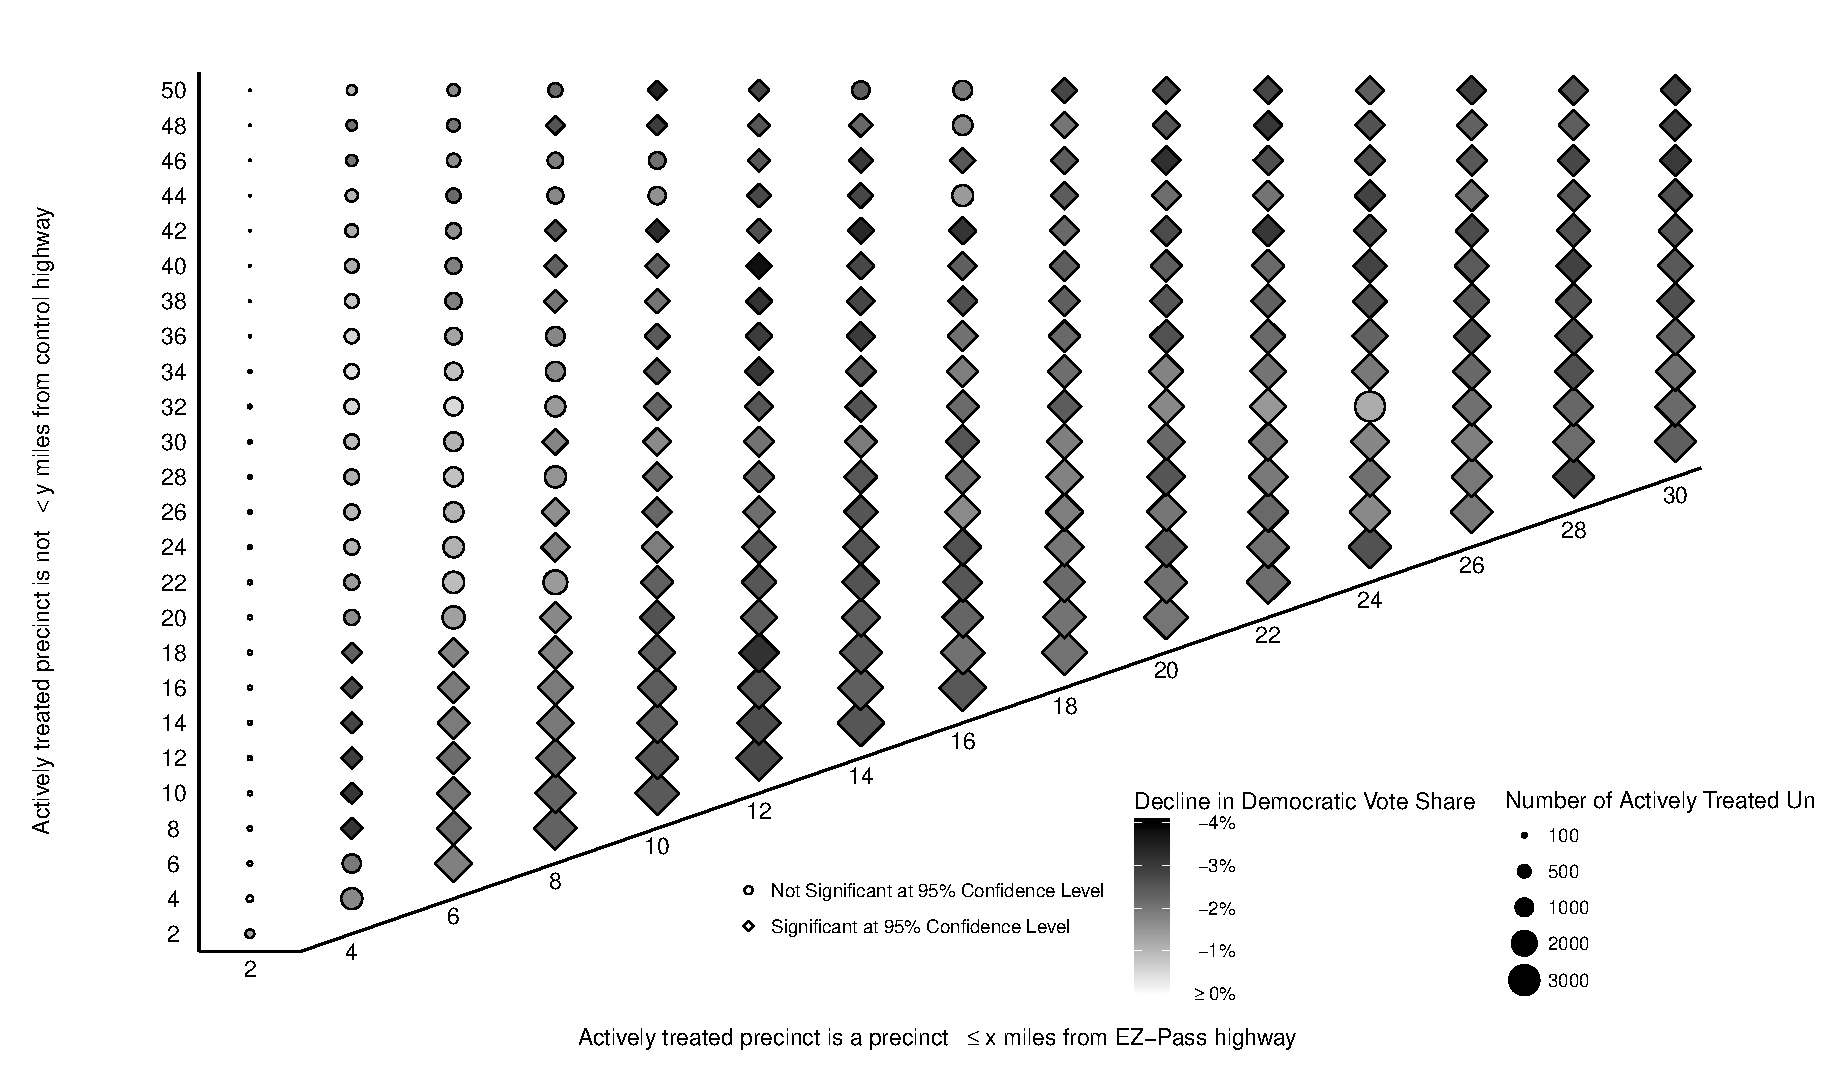
\includegraphics[width=0.9\textwidth]{Figures/new_style_04.eps}
    \caption{Sensitivity Analysis. $X$-$Y$ position gives the conditional difference in difference for a given combination of inclusion rule and exclusion rule. For example, at (12,18), one sees the effect of saying treated precincts are those within 12 miles of an E-ZPass highway but more than 18 miles from a non EZ-Pass highway, and similarly for control units. Effect size is indicated by the darkness of the shape, number of matched units is indicated by the area of the point, and results that are significant at the conventional 95\% threshhold are indicated by diamonds. Generally, effect magnitudes and significance are not sensitive to choice of rule, changes in effect magnitude are gradual.}
    \label{fig:heatmap}
\end{figure}

Any diff-in-diff analysis is also threatened by the presence of time-varying confounders. The effect of the E-ZPass intervention might be correlated with other changes occurring in treated or control communities. Although we have little leverage in directly identifying unobserved confounding, we can establish empirically whether key observed confounders might be changing along with our outcomes of interest. In particular, we can identify such effects by completing the same diff-in-diff procedure for other factors that are important for predicting Democratic vote share. We find that no key predictors of Democratic vote share underwent changes associated with the introduction of the E-ZPass. 

Table \ref{alt_explanations} shows that average incomes seem to have remained stable in treated E-ZPass precincts relative to their control counterparts. The diff-in-diff estimate ranges from -$\$613$ to -$\$1,450$, but are statistically insignificant. We might have been concerned that E-ZPass might have pushed out poor residents and led to an influx of richer ones. However, this worry seems unfounded. Indeed, the sign suggests that incomes fell in E-ZPass precincts relative to control areas. Next, since E-ZPass precincts are now more desirable, it could be that these communities experienced an influx of new, potentially more conservative residents. However, we find that, on average, E-ZPass communities did not see a population change compared to the control areas. Changes in turnout might be another confounding variable. If E-ZPass significantly increase or decreased turnout, inferences about the changes in the average Democratic vote share might be suspect. Here too, we find no effect of E-ZPass. Finally, we might wonder whether other characteristics of the E-ZPass communities were affected by the introduction of the electronic tolls. Could it be that E-ZPass communities experienced changes in racial or educational composition? No, neither the percentage of black residents nor the percentage of residents with a bachelor's degree changed in treated relative to control precincts. 

\begin{table}[!tbp] \centering 
\caption{Diff-in-diff results for other key variables.}
\resizebox{0.95\textwidth}{!}{
\begin{tabular}{@{\extracolsep{5pt}} ccccc} 
\\[-1.8ex]\hline 
\hline \\[-1.8ex] 
& \multicolumn{2}{c}{\emph{Baseline model}} & \multicolumn{2}{c}{\emph{With covariate adjustment}} \\
& \multicolumn{2}{c}{\textemdash} & \multicolumn{2}{c}{\textemdash} \\
\hline \\[-1.8ex] 
Dependent variable & DiD Estimate & (Block Bootstrap S.D.) & DiD Estimate & (Block Bootstrap S.D.) \\ 
\hline \\[-1.8ex] 
\emph{Average income} & -613.81 & (2488.12) & -1830.39 & (2572.56) \\ 
\emph{Population} & 30.88 & (30.17) & 15.27 & (32.61) \\ 
\emph{Turnout} & 0.72 & (0.79) & 0.61 & (0.82) \\ 
\emph{Percent with bachelors} & 0.64 & (0.37) & 0.56 & (0.43) \\ 
\emph{Percent black} & 0.47 & (0.35) & 0.59 & (0.33) \\ 
\hline \\[-1.8ex] 
\end{tabular} 
} 
 \label{alt_explanations} 
\end{table} 


A second threat to inference comes from time-varying \emph{unobserved} confounders. Although it is impossible to disprove the presence of these confounders, we can nevertheless gain some leverage on the problem by considering the placebo case of Ohio. Ohio did not replace its toll structures with E-ZPass electronic tolls until 2008. Thus, we can use Ohio as a placebo case to help identify whether areas near toll exits underwent a unique process of political change relative to non-toll areas. We know that there should be no estimated effect of E-ZPass in this period. If we were to identify such an effect, we would have evidence that time-varying unobserved factors are making precincts near toll exits more conservative than those near non-toll exits. However, using the same matching algorithm, inclusion/exclusion rule, and modeling approach, we find that no such effect is present. We find that precincts near exits that would adopt E-ZPass saw a negative change in their average housing values, and a positive (but insignificant) change in Democratic vote share. These factors support the contention that it is the E-ZPass alone (not time-varying unobserved confounders) which is accounting for the decrease in Democratic vote share. 

\begin{table}[!bp] \centering 
\resizebox{0.95\textwidth}{!}{%
\begin{tabular}{@{\extracolsep{5pt}} ccccc} 
\\[-1.8ex]\hline 
\hline \\[-1.8ex] 
Dependent variable & & DiD Estimate & (Bootstrap S.D.) & (Block Bootstrap S.D.) \\ 
\hline \\[-1.8ex] 
\multirow{2}{*}{\emph{Change in Average Home Price}} & Baseline model & \$-997 & (4,557) & (5,379) \\ 
& With covariate adjustment & \$3,358 & (4,382) & (5,038) \\ 

\multicolumn{5}{c}{\textemdash} \\ 
\multirow{2}{*}{\emph{Change in Democratic Vote Share}} & Baseline model & 1.39 & (0.53) & (0.68) \\ 
& With covariate adjustment & 0.74 & (0.87) & (0.8) \\ 
\hline \\[-1.8ex] 
\end{tabular} %
}
  \caption{Placebo analysis. Diff-in-diff results for change in average home price and Democratic vote share for Ohio.
          Matching/control variables include precinct-level covariates on average income, 
          percent of residents living in the same house as in 1995, percent of residents who are black, 
          percent of residents who are over the age of 65, percent of residents with a bachelor's degree. All matching/control data are from the US Census Bureau.}
  \label{placebo_voteshare_did} 
\end{table} 
One final threat to inferential validity is the possibility of unobserved confounders, a particularly serious problem when dealing with data that has a high degree of geographic correlation. While one cannot possibly hope to exhaust all such possible confounders, we do think it appropriate to consider one obvious confounder: weather. \textcite{Gomez2007} presents regression estimates of the effect of rain and snow on turnout and propoensity to vote Repbulican. They find that for every inch of rain above the normal amount of rain a place gets, there is on average about a 0.83\% in turnout and about a 2\% increase in Republican vote. Since weather is also spatially correlated, it has the potential to confound the estimates for our vote-share dependent variable, although not for our dependent variables based on donations. The perfect storm, so to speak, would be if it rained heavily along I-76 and I-95 (Southern Pennsylvania and Western New Jersey, respectively) in 2004, but nowhere else in 2004, and everywhere else in 2000. Fortunately, the perfect storm did not happen.  Figure \ref{fig:precipitation} presents precipitation maps from November 7th, 2000 and Nov 2nd, 2004 as reported by the National Oceanic and Atmospheric Administration (NOAA). According to these maps, on election day 2000 there was about $\nicefrac{1}{100^{\mathrm{th}}}$ an inch of precipitation in Western Pennsylvania, while on election day 2004 there was about $\nicefrac{1}{4^{\mathrm{th}}}$ of an inch of rain in Western Pennsylvania, about $\nicefrac{1}{10^{\mathrm{th}}}$ of an inch in Central Pennsylvania, and a touch of rain around New York City. This is not a great deal of rain. Historical data available through Weather Underground characterizes conditions in the apparent epicenter, Pittsburgh, as ``light rain" for most of the afternoon, cloudy in the morning and evening, with some additional rain around 9 PM. If one accepts the estimates in \textcite{Gomez2007}, the rain differential between 2004 and 2000 is not enough to make a significant dent in our estimates, even in a worst case analysis.\footnote{The normal rainfall in Pennsylvania is about 0.1 inches, so a worst case analysis that assumes 0.3 inches of rain in every treated unit but a normal amount of rain in every control would still only explain a 0.4\% increase in Republican vote. The effect we found was an order of magnitude larger. }  Moreover, the rain appears to affect treated and control regions evenly in 2004, if anything control regions were hit harder. To be especially sure that rain has not interfered our inference, we estimate the effect on turnout due to EZ-Pass.  We find that there was no significant effect on turnout, which one would expect if rain was a serious confounder, and indeed the sign goes the opposite direction.

\begin{figure}[t]
    \centering
    \begin{subfigure}[b]{0.45\textwidth}
        \includegraphics[width=\textwidth]{Figures/Election_2000_wednesday.png}
        \caption{7AM Nov. 7 - 7AM Nov. 8, 2000}
        \label{fig:gull}
    \end{subfigure}
    ~ %add desired spacing between images, e. g. ~, \quad, \qquad, \hfill etc. 
      %(or a blank line to force the subfigure onto a new line)
    \begin{subfigure}[b]{0.45\textwidth}
        \includegraphics[width=\textwidth]{Figures/precip_20041103.png}
        \caption{7AM Nov. 2 - 7 AM Nov. 8, 2000}
        \label{fig:tiger}
    \end{subfigure}
    \caption{National weather maps from the two election days used in our study (Source: National Oceanic and Atmospheric Administration Central Library Data Imaging Project). The chart shows areas that had precipitation during the 24 hour period starting at 7 AM EST the day indicated until 7AM EST the next day. All numbers are reported in inches rounded to the nearest $\nicefrac{1}{100^{\mathrm{th}}}$, except for \textbf{.T} which refers to trace amounts of precipitation.}\label{fig:precipitation}
\end{figure}